\documentclass{beamer}


% Theme and page layout
\usetheme{gapz}
\setbeamertemplate{navigation symbols}{}

% Fonts
\usepackage{fontspec}
\defaultfontfeatures{Mapping=tex-text,Scale=MatchLowercase,Numbers=Lining}
%\setsansfont[
%	ItalicFont = Whitney MediumItalic,
%	BoldFont = Whitney Semibold,
%	BoldItalicFont = Whitney SemiboldItalic,
%	SmallCapsFont = Whitney MediumSC
%]{Whitney Medium}

% Language
\usepackage{polyglossia}
\setdefaultlanguage{english}

% Graphics
\usepackage{graphicx}
\graphicspath{{./images/}}



\title{Three-dimensional modeling and printing project}
\subtitle{}
\author[V. D., A. L., C. N., J. P., F. R.]{\begin{scriptsize}
Vincent~Duvert \\ Antoine~Lubineau \\ Caroline~Naud \\ James~Packer \\ Florian~Ribon\end{scriptsize}}
\date{from January 23 to March 16, 2012}

\titlegraphic{
\includegraphics[width=4cm]{inp-enseeiht}}

\begin{document}

\frame{\titlepage}

\section{Presentation of the project}

\subsection{The client team}
\begin{frame}
	\frametitle{The client team}
	
	\begin{block}{The \textsc{VORTEX} team of IRIT}
		\begin{itemize}
		\item \textsc{IRIT} : a research institute in computer science from Toulouse
		\item \textsc{VORTEX} : Visual Objects : from Reality To EXpression
		\item skills in the areas of graphic computing,  computer vision, artificial intelligence and networks
		\item recently acquired an Ultimaker 3D printer on which she has no control over
		\end{itemize}
    \end{block}
    
    \begin{center}
		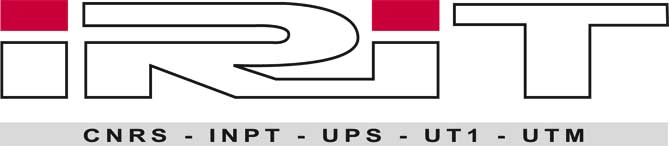
\includegraphics[width=4cm]{irit}	
	\end{center}
    
\end{frame}

\subsection{The resources}
\begin{frame}
	\frametitle{The resources}
	
	\begin{block}{The project team}
		\begin{itemize}
		\item Five final year students at ENSEEIHT, Computing and Applied Mathematics department, interested in using the printer
		\end{itemize}
    \end{block}
    
    \begin{block}{The material resources}
    	\begin{itemize}
		\item room F117 in building F at ENSEEIHT
    	\item Ultimaker 3D printer with a roll of PLA plastic
    	\item computer with dual-touch screen Acer T231H
    	\item computer rooms of the ENSEEIHT and personnal computer
		\end{itemize}
    \end{block}
      
\end{frame}

\begin{frame}
	\frametitle{Ultimaker 3D printer}

    \begin{center}
		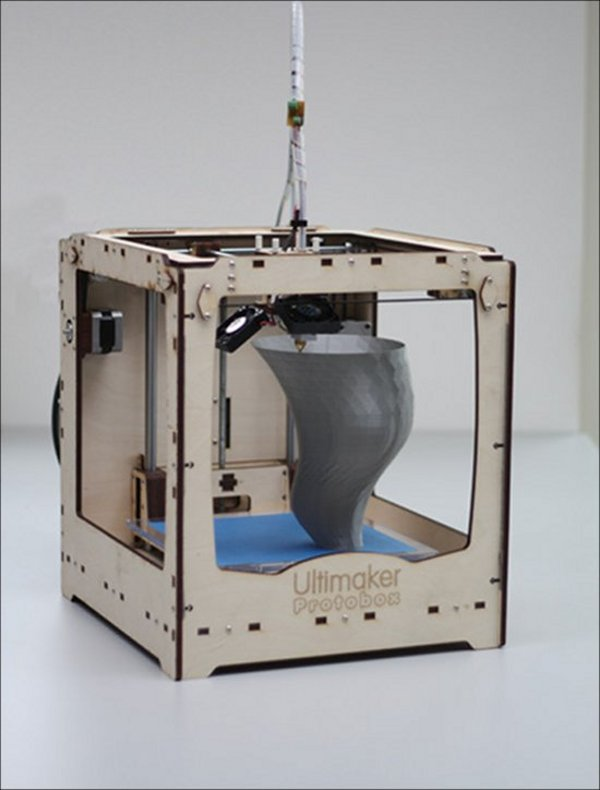
\includegraphics[width=4cm]{Ultimaker}	
	\end{center}
    
\end{frame}

\subsection{The objectives}
\begin{frame}
	\frametitle{The main client's requests}
	\begin{block}{Main goals of the project} 
	\begin{itemize}	
		\item development of a fully open-source software with graphical interface that allows to import, model and deform virtual 3D objects, preferably using a dualtouch screen
		\item export of the corresponding meshes to the printer to finally print it as realistically as possible.
	\end{itemize}
    \end{block}
    
    \begin{block}{The final users}
    	\begin{itemize}
		\item The \textsc{VORTEX} team
		\item Some artists from Artilect for example (or artists students)
		\end{itemize}
    \end{block}
    
\end{frame}

\section{About the project management ...}
\begin{frame}
	\frametitle{The V cycle management strategy}

    \begin{center}
		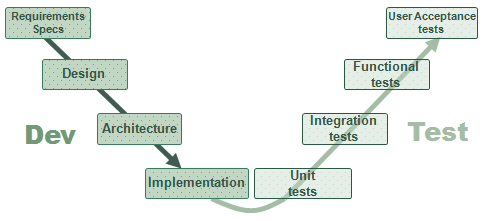
\includegraphics[width=8cm]{VCycle}	
	\end{center}
\end{frame}

\section{Architecture of the project}
\begin{frame}
	\frametitle{blabla}

    \begin{center}
		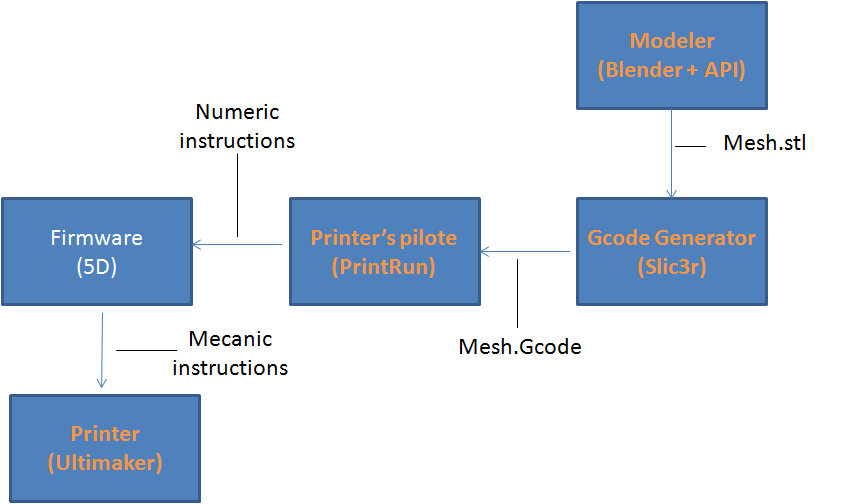
\includegraphics[width=8cm]{ARD1}	
	\end{center}
	
\end{frame}

\section{Mesh correction}
\begin{frame}
	\frametitle{blabla}

    \begin{block}{blabla}
    \end{block}
\end{frame}

\section{Modifications in Blender's interface}
\begin{frame}
	\frametitle{blabla}

    \begin{block}{blabla}
    \end{block}
\end{frame}

\section{Calibration of the printer}
\begin{frame}
	\frametitle{blabla}

    \begin{block}{blabla}
    \end{block}
\end{frame}

\section{Conclusions and thanks}
\begin{frame}
	\frametitle{blabla}

    \begin{block}{blablabla}
    \end{block}
\end{frame}

\begin{frame}
	\frametitle{}

    \begin{center}
    \Large{Thank you for your attention !}
    \end{center}
\end{frame}
	
\end{document}
